\documentclass[11pt,a4paper]{article}
\usepackage[czech]{babel}
\usepackage[utf8]{inputenc}
\usepackage[T1]{fontenc}
\usepackage[top=2.5cm, left=2cm, text={17cm, 25cm}]{geometry}
\usepackage{graphicx}
\usepackage{caption}
\usepackage{subcaption}
\usepackage{amsmath}
\usepackage{multirow}
\usepackage[bookmarksopen,colorlinks,plainpages=false,urlcolor=blue,unicode]{hyperref}
\usepackage{url}
\usepackage{listings}
\begin{document}

\def\authorv{Vojtěch Bartl}
\def\emailv{xbartl03@stud.fit.vutbr.cz}
\def\authorf{Pavel Frýz}
\def\emailf{xfryzp00@stud.fit.vutbr.cz}
\def\projname{Řešení prohibiční krize v~ČR}
\begin{titlepage}

% \vspace*{1cm}
\begin{figure}[!h]
  \centering
  
\includegraphics[height=5cm]{logo}
\end{figure}

\vfill

\begin{center}
\begin{Large}
Dokumentace k~projektu z~předmětu IMS\\
\end{Large}
\bigskip
\begin{Huge}
\projname\\
\end{Huge}
\end{center}

\vfill

\begin{center}
\begin{Large}
\today
\end{Large}
\end{center}

\vfill

\begin{flushleft}
\begin{large}
\begin{tabular}{ll}
Autor: & \authorv, \url{\emailv} \\
 & \authorf, \url{\emailf} \\
 & Fakulta informačních technologií \\
 & Vysoké učení technické v~Brně \\
\end{tabular}
\end{large}
\end{flushleft}
\end{titlepage}


\tableofcontents
\newpage

\section{Úvod}
V~této práci je řešena implementace modelu, který je určen pro stanovení 
nákladů na testování alkoholu prováděných Státní zemědělskou a potravinářskou inspekcí.
Smyslem experimentů je ověřit, jestli by se vyplatilo pořídit inspektorům
Ramanův spektrometr, pomocí něhož by inspektoři testovali vzorky na místě inspekce
a do laboratoře by se posílaly pouze podezřelé vzorky. Problém je zkoumán 
z~hlediska nákladů na testy a časového vytížení laboratoře. Při pořízení spektrometrů
bylo očekáváno snížení nákladů a zrychlení analýzy vzorků v~laboratoři. V~jednotlivých
testech byl zkoumán vliv počtu spektrometrů na chování systému. Po zjištěných výsledcích
byla do modelu přidána možnost umístění spektrometrů do laboratoří a stanovení
nákladů s~tímto nastavením.   

\subsection{Zúčastněné osoby}
Autory projektu jsou Vojtěch Bartl a Pavel Frýz. K~realizaci projektu dále přispěli
Dr. Ing. Petr Peringer, který vysvětlil principy diskrétní simulace a uvedl
základní znalosti potřebné pro řešení projektu a Ing. Martin Hrubý, Ph. D., který 
předvedl modelování systému hromadné obsluhy pomocí Petriho sítí a implementaci
pomocí knihovny SIMLIB.

\subsection{Validita modelu}
Chování modelu s~počátečními hodnotami bylo prověřeno porovnáním výsledků s~přepokládanými hodnotami,
které byly získány z~provedených kontrol Státní zemědělskou a potravinářskou inspekcí za období
od 7. září do 30. listopadu 2012.
 
\section{Rozbor tématu a použitých metod/technologií}
V~reakci na metanolovou aféru zvýšila Státní zemědělská a potravinářská inspekce
počet kontrol alkoholu. V~terénu provadí kontrolu všech 215 inspektorů. Pokud
inspekce odhalí podezřelou lihovinu, okamžitě odebere vzorek k~otestování \cite{szpi}. Od 7. září
do 30. listopadu 2012 bylo vykonáno 33 240 kontrol v~prodejnách, u~výrobců a v~místech, kde 
se čepují rozlévané lihoviny, vývoj počtu zkontrolovaných prodejen v~tomto období
můžete vidět na obrázku \ref{kontrol}. V~rámci kontrol odebrali inspektoři 889 vzorků. Po provedené analýze
bylo 785 vzorků vyhovujících a 42 nevyhovujících, vývoj počtu viz obrázek \ref{vzorky}~\cite{eagri}. Analýza jednoho vzorku 
trvá přibližně půl hodiny \cite{an1,an2,an3}. Náklady za rozbory prováděné laboratořemi 
Státní zemědělské a potravinářské inspekce jsou dle ceníku 950 Kč \cite{nak1}. 
Na území České republiky se nalézá 14 laboratoří s~akreditací na stanovení obsahu metanolu. 
Z~nichž 2 provozuje Státní a potravinářská inspekce \cite{akre}.

\begin{figure}[h!]
  \centering
  \begin{subfigure}[t]{0.5\textwidth}
    \centering
    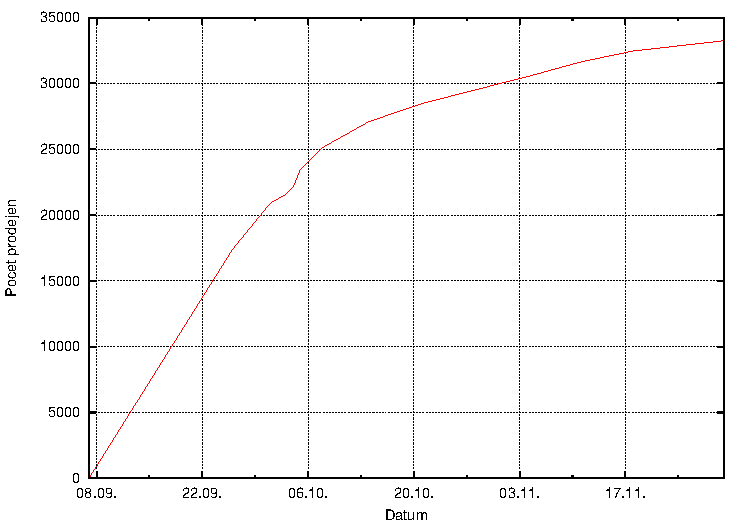
\includegraphics[width=\textwidth]{kontrol}
    \caption{Počet kontrol}
    \label{kontrol}
  \end{subfigure}%
  ~ %add desired spacing between images, e. g. ~, \quad, \qquad etc. 
  %(or a blank line to force the subfigure onto a new line)
  \begin{subfigure}[t]{0.5\textwidth}
    \centering
    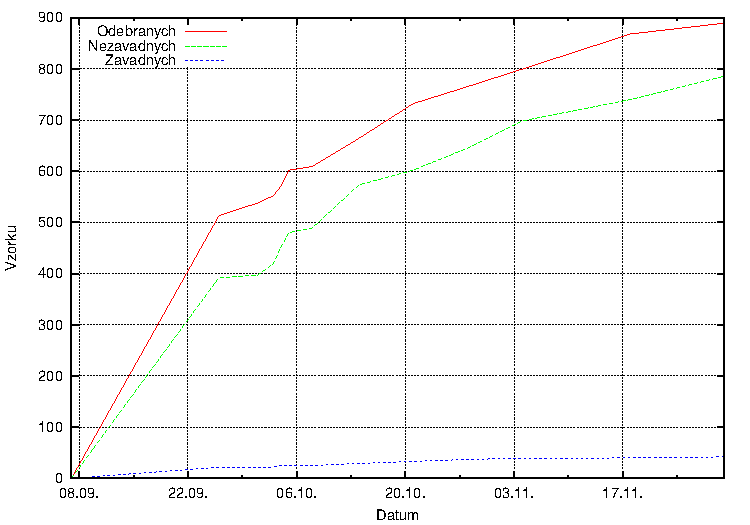
\includegraphics[width=\textwidth]{vzorky}
    \caption{Počet vzorků}
    \label{vzorky}
  \end{subfigure}
  \caption{Průběh inspekcí}
\end{figure}

Vysoká škola chemicko-technologická v~Praze vyvinula způsob, jak zjistit
koncetraci metanolu, ke stanovení obsahu využívá Ramanův spektrometr. Metoda není 
v~současné době certifikována. Náklady na otestování jednoho vzorku touto metodou vyjdou 
na desítky korun a trvají v~řádu minut \cite{raman1,raman2}. Pořizovací cena Ramanova spektrometru 
je zhruba 0,75 milionu korun. \cite{rcen}. 

\subsection{Popis použitých postupů, metod a technologií}
Systém [IMS 7/329] je převeden na abstraktní model [IMS 43/329].
Model je vyjádřen pomocí Petriho sítě [IMS 63/329] a následně
je abstrakní model převeden na simulační model [IMS 46/329],
simulační model je napsán v~jazyce C++ s~využitím
knihovny SIMLIB. Implementační jazyk a knihovna byly zvoleny podle
toho, že se jedná o~systém hromadné obsluhy [IMS 139/329]. Implementace
systému hromadné obsluhy užitím knihovny SIMLIB je snadná a byla nám doporučena v~rámci
demonstračních cvičení, které vedl Ing. Martin Hrubý, Ph. D..
Sledovanými vlastnostmi systému hromadné obsluhy bývá doba strávená v~systému, čas čekání ve frontách a 
vytížení obslužných linek. Cílem sytémů hromadné obsluhy bývá například optimalize výkonu. V~našem případě je 
obslužnou linkou laboratoř, která přijímá vzorky od inspektorů a provádí jejich
analýzu.

\section{Koncepce}
Inspektor provádí inspekce v~prodejnách. V~případě, kdy má inspektor
Ramanův spektrometr, provede po skončení inspekce test odebraných
vzorků. Odebrané vzorky posílá inspektor na konci svého pracovního dne 
do laboratoře. Předpokládáme pracovní dobu
inspektora 8 hodin. Z~počtu vykonaných inspekcí za období
7. 9.\,--\,30. 11. 2012, předpokládáme průměrnou dobu inspekce 4 hodiny.
Předpokladáme odebrání vzorků z~1\% prodejen, vycházíme z~počtu
provedených kontrol a odebraných vzorů, a z~přepokladu odebrání
více vzorků z~jedné prodejny. Spektrometr si bere inspektor ze skladu
před započetím inspekce. Spektrometr vrací do skladu na konci své pracovní doby.

Laboratoř poté provádí testování vzorků a rozdělení na nezávadné a závadné.
Předpokládáme, že laboratoř je v~provozu 16 hodin denně.
Předpokládáná doba jednoho testu je průměrně 30 minut. Předpokládaný počet
závadných vzorků je 5\%, odvozeno z~poměru nezávadných a závadných vzorků.

Na obrázku \ref{petriner} je uvedeno zjednodušené schéma systému. Schéma
zobrazuje práci inspektora, odebírání vzorků, případný rozbor vzorků pomocí
spektrometru, odeslání vzorků do laboratoře a následnou analýzu v~laboratoři. 
Vzorky jsou při odesílání inspektorem do laboratoře rozděleny podle toho jestli 
byly analyzovány spektrometrem. 

Předpokládané náklady na rozbor vzorku v laboratoří činí 950 Kč, za rozbor
vzorku spektrometrem 25 Kč, pořizovací cena spektrometru 750 000 Kč. 


  \begin{figure}[h!]
    \centering
    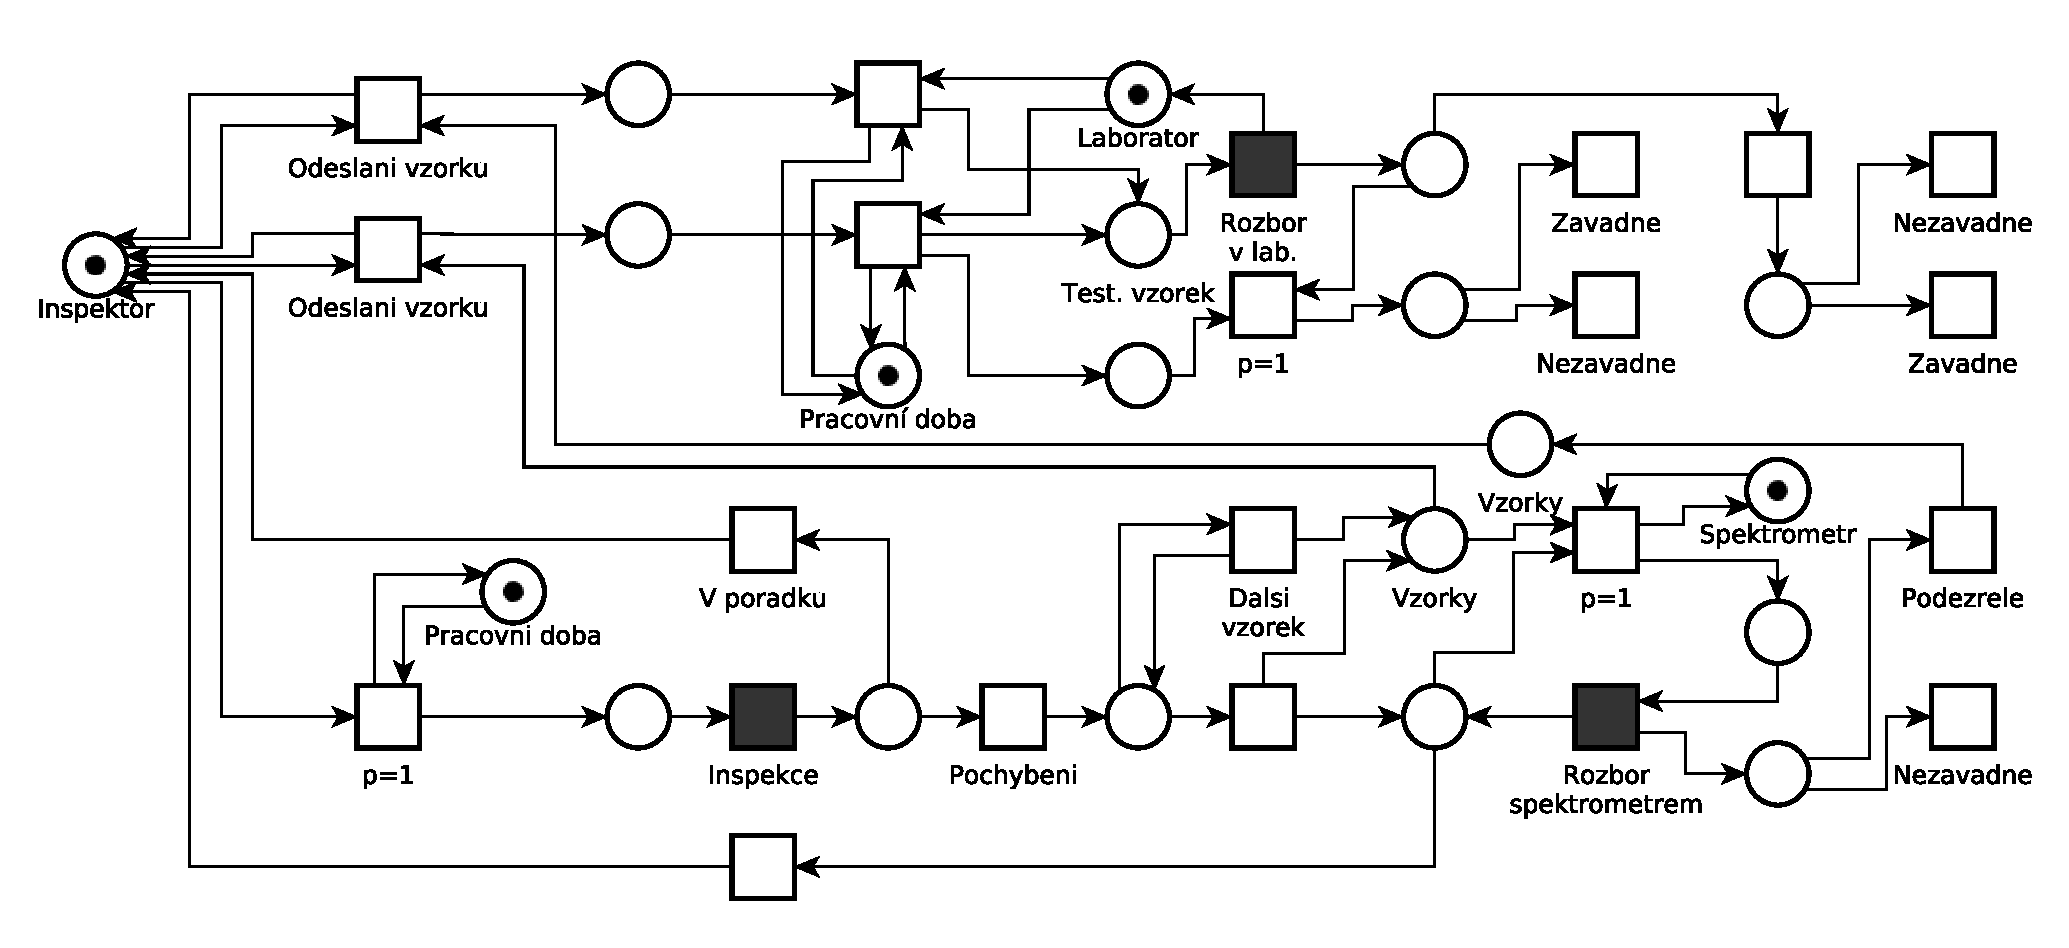
\includegraphics[width=0.8\textwidth]{petri}
    \caption{Schéma systému}
    \label{petriner}
  \end{figure}

\section{Architektura simulačního modelu/simulátoru}
K~implementaci modelu byl použit jazyk C++ a knihovna SIMLIB.
Program funguje jako konzolová aplikace. Překlad programu se provede
příkazem \texttt{make}. Spuštění se provede příkazem \texttt{make run},
kdy se provede několik experimentů s~různými parametry programu a výsledky
se uloží do souborů, z~dat výsledku lze vytvořit grafy příkazem \texttt{make plot}.

\subsection{Mapování abstraktního modelu do simulačního}
V~programu byla implementována třídy \texttt{LabTimer} a \texttt{WorkTimer},
které řídí pracovní dobu inspektora, resp. provozní dobu laboratoře.
Dále byla vytvořena třída \texttt{Inspektor}, jedná se o~proces inspektora,
provádí se v~něm inspekce provozoven, odebírání vzorků inspektorem, případná 
analýza spektrometrem a odesílání vzorků do laboratoře. Třída \texttt{Laboratory}
reprezentující laboratoř. Dále je implementována třída \texttt{Sample}, jedná se
o~proces řídící zpracování vzorku v~laboratoři, provádí se v~něm zabrání zařízení laboratoře, analýza vzorku
a následné uvolnění zařízení.

\section{Podstata simulačních experimentů a jejich průběh}
\subsection{Obecný popis experimentů}
Následující experimenty se zabývají vlivem nastavení hodnot systému
na náklady spojené s~analýzou vzorků. Dále se zabývají počtem
odebraných vzorků a dobou vzorků strávených v~laboratoři do jejich
vyhodnocení.
\subsection{Prováděné experimenty}
\subsubsection*{Chování systému s~počátečními hodnotami}
Počáteční hodnoty byly zvoleny, tak aby odpovídaly reálným
hodnotám a mohli jsme porovnat výsledek s~očekávaným výsledkem.
Počet Inspektorů byl nastaven na 215, což je počet inspektorů
SZPI, počet laboratoří byl nastaven na 2, podle počtu laboratoří
vlastněných SZPI. Jelikož SZPI při testování nepoužívá Ramanův
spektrometr, byl počet spektrometrů nastaven na 0. Doba simulace
byla nastavena na 84 dní, tj. počet dní od 7. září do 30. listopadu 2012.
Výsledek zatížení laboratoří můžete vidět na obrázku \ref{init},
který znázorňuje dobu, která byla potřeba od přijetí vzorku do laboratoře po ukončení
jeho analýzy. Na grafu je vidět, že nejvíce vzorků je vyhodnoceno přibližně za 30 minut.
Na grafu dále vidíme hroty vzdálené od sebe 30 minut. Které jsou způsobené přijetím
více vzorku od jednoho inspektora a postupným zpracováním těchto vzorků. Klesající
tendence hrotů kopíruje exponenciální rozložení počtu odebraných vzorků inspektorem. Od 7 hodin můžeme
vidět nárust počtu vzorků, jedná se o~vzorky, které byli přijaty v~době, kdy
laboratoř nebyla v~provozu. V~tabulce \ref{tabinit} pak můžete vidět počet
zkontrolovaných prodejen, odebraných vzorků, počet závadných a nezávadných vzorků a 
celkové náklady. 

  \begin{figure}[h!]
    \centering
    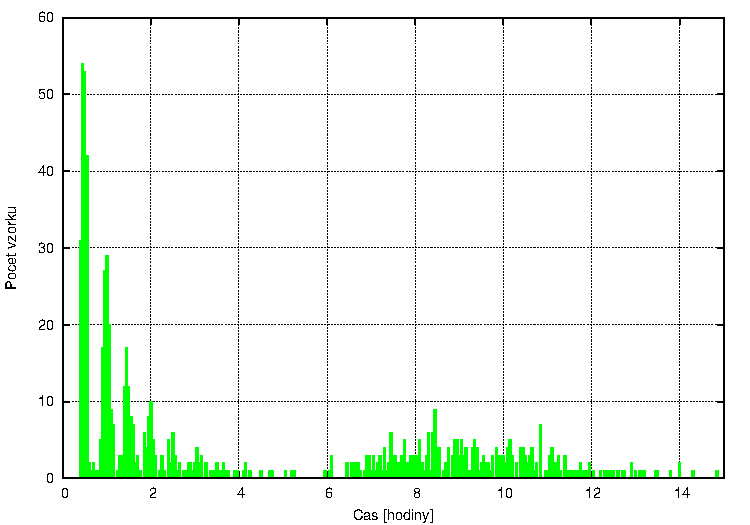
\includegraphics[width=0.7\textwidth]{init}
    \caption{Zatížení laboratoře s~počátečními hodnotami}
    \label{init}
  \end{figure}
  
  \begin{table}[h!]
    \catcode`\-=12
    \begin{center}
      \begin{tabular}{|r|r|r|r|r|r|}  \hline
        \textbf{Prodejen} & \textbf{Vzorků} & \textbf{Závadných}   
        & \textbf{Nezávadných} & \textbf{Náklady [Kč]} \\\hline
        31 097&783&746&30&737 200         \\\hline
      \end{tabular}
      \caption{Výsledky systému s~počátečními hodnotami}
      \label{tabinit}
    \end{center}
  \end{table} 
\vfill
\subsubsection*{Vliv počtu spektrometrů na chování systému}
Následující experimenty se zabývaly vlivem počtu spektrometrů,
které mají inspektoři k~dispozici, na chování systému. Experimenty byly
provedeny s~počtem inspektorů 200 a 500, analýza vzorků probíhala v~jedné 
laboratoři. Čas simulace byl nastaven na 180 dní. Počet spektrometrů byl
nastaven na 0, 1/4 počtu inspektorů, 1/2 počtu inspektorů a pro každého
inspektora jeden. Výsledek s~nulovým počtem inspektorů můžete vidět na obrázcích
\ref{zeroa}, \ref{zerob}. Pokud výsledné histogramy porovnáme, vidíme, že jsou
si velmi podobné, hlavním rozdílem je změna měřítka na ose y, histogram je také
velmi podobný histogramu s~původními hodnotami. Změna měřítka je způsobena
změnou délky experimentu a počtem inspektorů, které má za následek vygenerování
více vzorků k~otestování.

\begin{figure}[h!]
  \centering
  \begin{subfigure}[t]{0.5\textwidth}
    \centering
    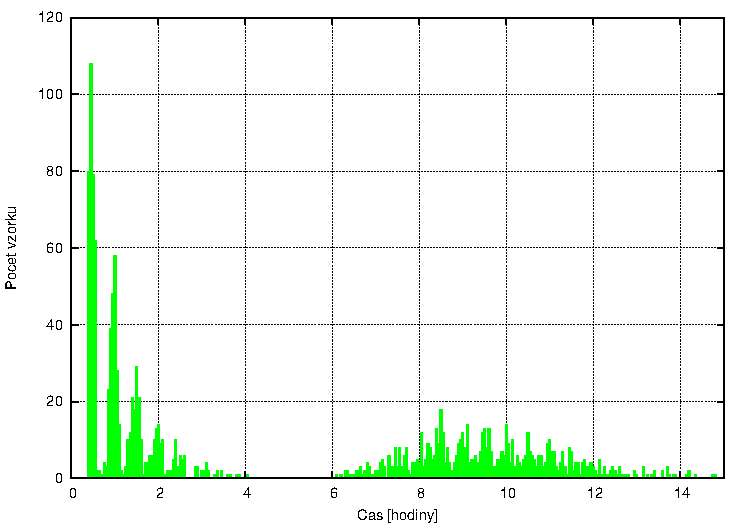
\includegraphics[width=\textwidth]{exp1_200}
    \caption{200 Inspektorů}
    \label{zeroa}
  \end{subfigure}~\begin{subfigure}[t]{0.5\textwidth}
    \centering
    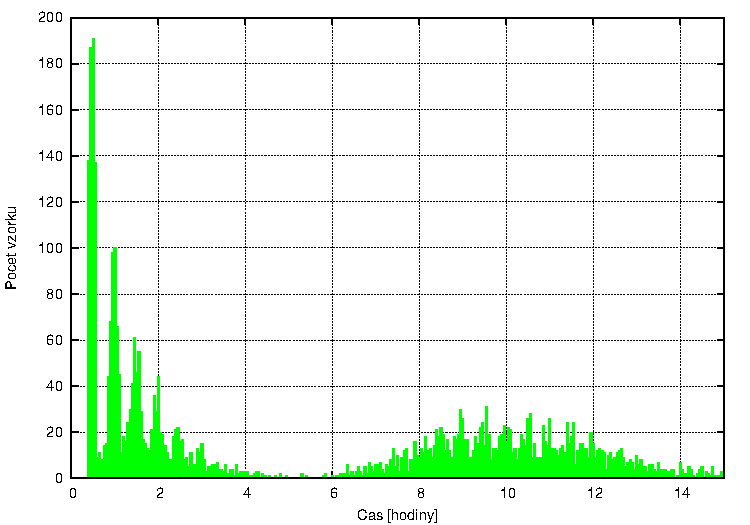
\includegraphics[width=\textwidth]{exp1_500}
    \caption{500 Inspektorů}
    \label{zerob}
  \end{subfigure}
  \begin{tabular}{|r|r|r|r|r|r|}  \hline
        \textbf{Inspektorů}&\textbf{Prodejen} & \textbf{Vzorků} & \textbf{Závadných}   
        & \textbf{Nezávadných} & \textbf{Náklady [Kč]} \\\hline
        \textbf{200}&61 812&1 502&1 404&98&1 426 900         \\\hline
        \textbf{500}&154 811&3 910&3 727&178&3 709 750         \\\hline
      \end{tabular}
  \caption{Výsledky systému s~nula spektrometry}
\end{figure} 


Na grafech \ref{quarta}, \ref{quartb} vidíme průběh při zakoupení
spektrometrů odpovidájící 1/4 počtu inspektorů, tj. 50 spektrometrů, resp.
125 spektrometrů. Oproti předcházejícímu případu, kdy inspektoři neměli žádný spektrometr,
vidíme na grafu úbytek vzorků, způsobený tím, že někteřé vzorky nejsou
vůbec zasláný do laboratoře, jelikož jsou zkontrolovány na místě pomocí spektrometru.
Dále můžeme vidět zvětšení poměru mezi jednotlivými hroty, nejlépe viditelné u~prvního 
a druhého hrotu, způsobené tím, že inspektor neposílá tolik vzorků naráz.

\begin{figure}[h!]
  \centering
  \begin{subfigure}[t]{0.5\textwidth}
    \centering
    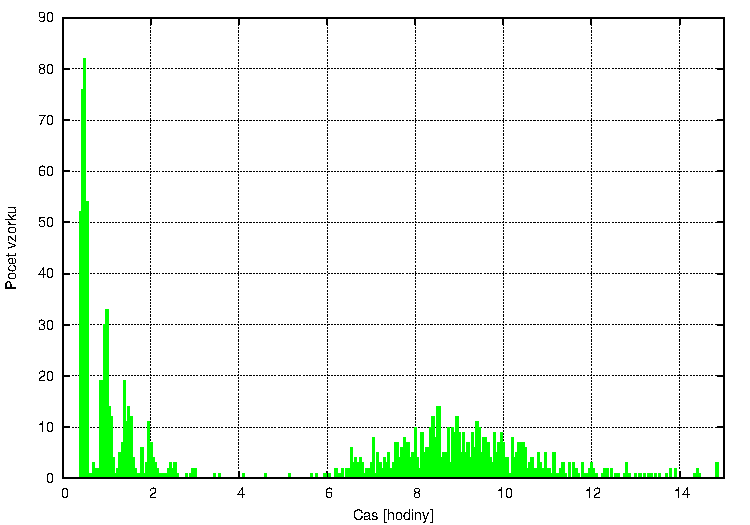
\includegraphics[width=\textwidth]{exp2_200}
    \caption{200 Inspektorů}
    \label{quarta}
  \end{subfigure}~\begin{subfigure}[t]{0.5\textwidth}
    \centering
    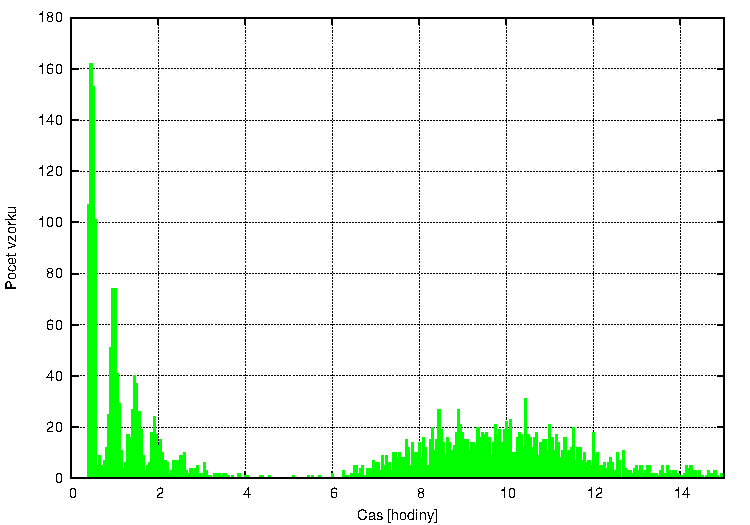
\includegraphics[width=\textwidth]{exp2_500}
    \caption{500 Inspektorů}
    \label{quartb}
  \end{subfigure}
  \begin{tabular}{|r|r|r|r|r|r|}  \hline
        \textbf{Inspektorů}&\textbf{Prodejen} & \textbf{Vzorků} & \textbf{Závadných}   
        & \textbf{Nezávadných} & \textbf{Náklady [Kč]} \\\hline
        \textbf{200}&61 761&1 537&1 468&69&38 597 725         \\\hline
        \textbf{500}&154 771&3 777&3 584&184&96 593 000         \\\hline
      \end{tabular}
  \caption{Výsledky systému se čtvrtinou spektrometrů}
\end{figure} 

Na grafech \ref{halfa}, \ref{halfb} můžeme vidět průběh při zakoupení spektrometrů
odpovídající 1/2 počtu inspektorů. Změna jsou velmi podobné předcházejícímu případu.
Došlo ještě většímu snížení vzorků a zvýšení poměru jednotlivých hrotů.
Zajímavé je vystoupení hrotů v~pozdějších hodinách, které na předchozích grafech nebyly
tak výrazné.

\begin{figure}[h!]
  \centering
  \begin{subfigure}[t]{0.5\textwidth}
    \centering
    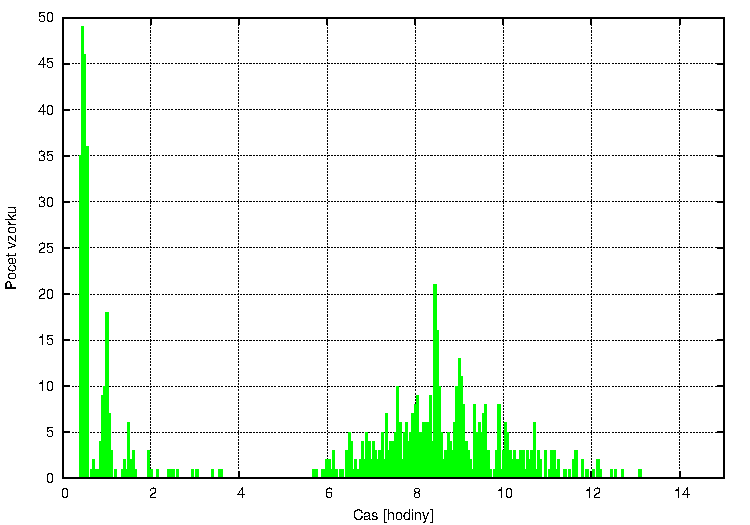
\includegraphics[width=\textwidth]{exp3_200}
    \caption{200 Inspektorů}
    \label{halfa}
  \end{subfigure}~\begin{subfigure}[t]{0.5\textwidth}
    \centering
    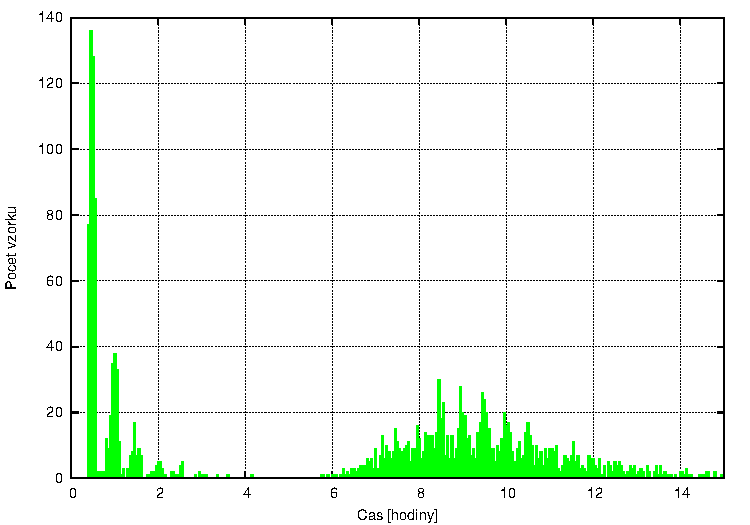
\includegraphics[width=\textwidth]{exp3_500}
    \caption{500 Inspektorů}
    \label{halfb}
  \end{subfigure}
  \begin{tabular}{|r|r|r|r|r|r|}  \hline
        \textbf{Inspektorů}&\textbf{Prodejen} & \textbf{Vzorků} & \textbf{Závadných}   
        & \textbf{Nezávadných} & \textbf{Náklady [Kč]} \\\hline
        \textbf{200}&61 875&1 472&1 400&66&75 700 150         \\\hline
        \textbf{500}&154 600&3 860&3 660&194&189 390 825         \\\hline
      \end{tabular}
      \caption{Výsledky systému se půlkou spektrometrů}
\end{figure} 

Průběh při zakoupení spektrometrů odpovídající počtu inspektorů můžeme vidět na
grafech \ref{fulla}, \ref{fullb}. Zde je vidět, že do laboratoře se posílá
velmi malý počet vzorků a nebýt toho, že laboratoř má určitou pracovní
dobu, byly by skoro všechny vzorky vyhodnoceny během první hodiny.

\begin{figure}[h!]
  \centering
  \begin{subfigure}[t]{0.5\textwidth}
    \centering
    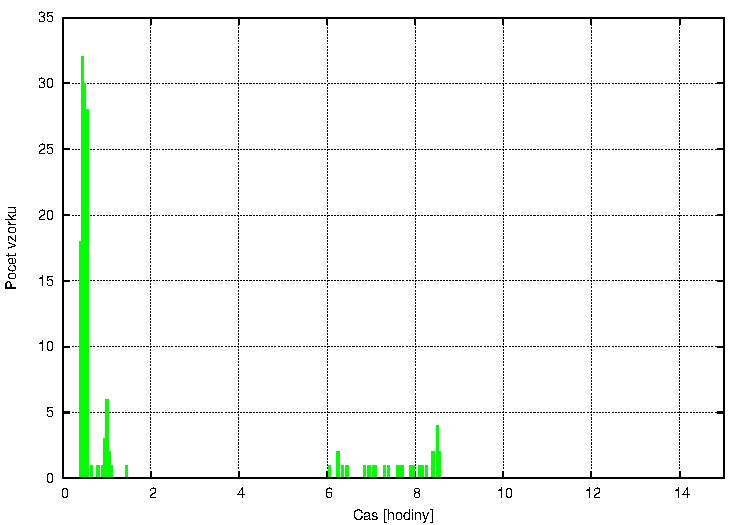
\includegraphics[width=\textwidth]{exp4_200}
    \caption{200 Inspektorů}
    \label{fulla}
  \end{subfigure}~\begin{subfigure}[t]{0.5\textwidth}
    \centering
    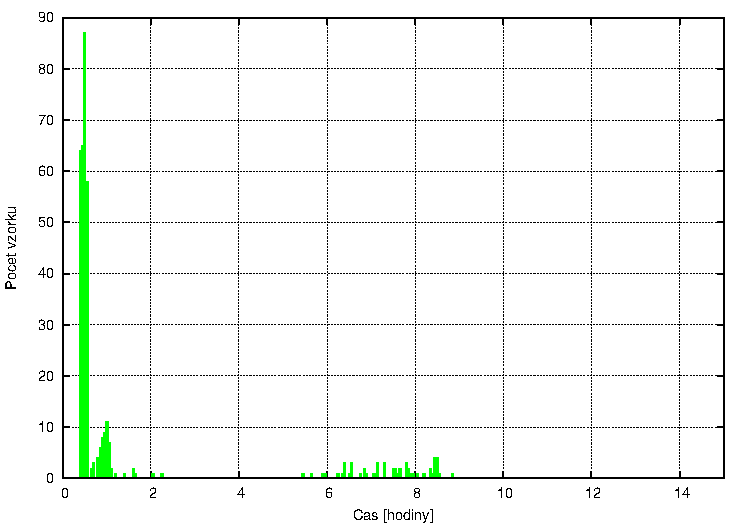
\includegraphics[width=\textwidth]{exp4_500}
    \caption{500 Inspektorů}
    \label{fullb}
  \end{subfigure}
  \begin{tabular}{|r|r|r|r|r|r|}  \hline
        \textbf{Inspektorů}&\textbf{Prodejen} & \textbf{Vzorků} & \textbf{Závadných}   
        & \textbf{Nezávadných} & \textbf{Náklady [Kč]} \\\hline
        \textbf{200}&61 817&1 393&1 320&73&150 178 275         \\\hline
        \textbf{500}&154 414&3 891&3 683&208&375 464 925         \\\hline
      \end{tabular}
      \caption{Výsledky systému se počtem spektrometrů odpovídajícím počtu inspektorů}
\end{figure} 

\subsubsection*{Vliv spektrometru v~laboratoři na chování systému}
Nástavení systému bylo stejné jako v~předcházejích experimentech. 
Inspektoři, ale neměli žádný spektrometr, naopak v~laboratoři jeden byl.
Výsledky můžete vidět na grafech \ref{speca}, \ref{specb}. Nejzajímavější
je porovnání s~grafy \ref{zeroa} a \ref{zerob}, jelikož systémy se liší
pouze jedním spektrometrem, který je umístěn v~laboratoři. Počet
zpracovávaných vzorků je tedy víceméně stejný. Zpracování vzorků 
v~laboratoří se spektrometrem je několikanásobně rychlejší.

\begin{figure}[h!]
  \centering
  \begin{subfigure}[t]{0.5\textwidth}
    \centering
    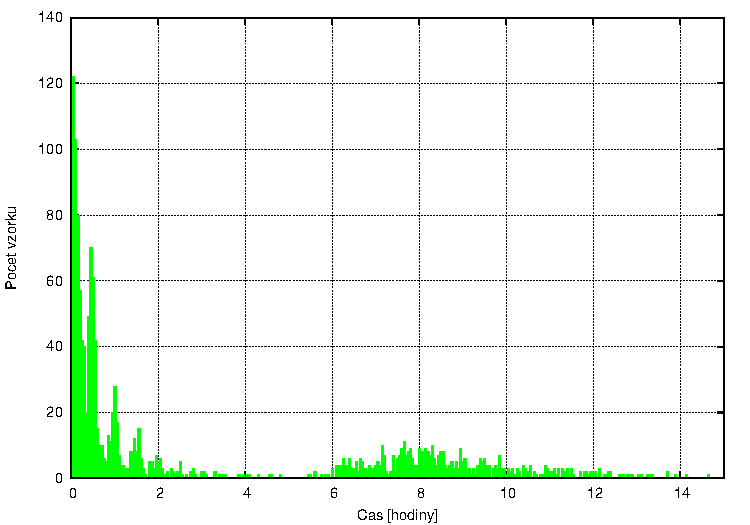
\includegraphics[width=\textwidth]{exp5_200}
    \caption{200 Inspektorů}
    \label{speca}
  \end{subfigure}~\begin{subfigure}[t]{0.5\textwidth}
    \centering
    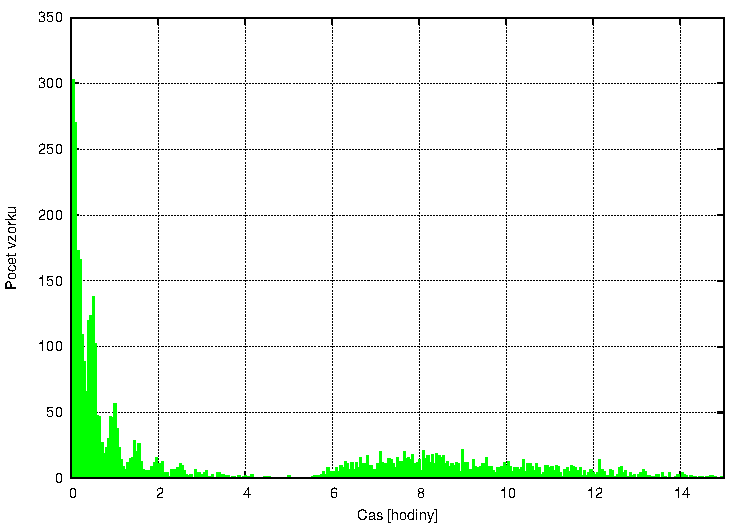
\includegraphics[width=\textwidth]{exp5_500}
    \caption{500 Inspektorů}
    \label{specb}
  \end{subfigure}
 \begin{tabular}{|r|r|r|r|r|r|}  \hline
        \textbf{Inspektorů}&\textbf{Prodejen} & \textbf{Vzorků} & \textbf{Závadných}   
        & \textbf{Nezávadných} & \textbf{Náklady [Kč]} \\\hline
        \textbf{200}&61 798&1 481&1 405&76&1 546 575         \\\hline
        \textbf{500}&154 736&3 956&3 745&208&2 777 775         \\\hline
      \end{tabular}
      \caption{Výsledky systému se jedním spektrometrem v~laboratoři}
\end{figure} 
  
\subsection{Závěry experimentů}
Bylo provedeno 11 experimentů s~různým počtem inspektorů a Ramanových spektrometrů.
V~průběhu testování byl model rozšířen o~možnost vyhodnocení nákladů při umístění
spektrometrů do laboratoří, vedly nás k~tomu výsledky z~předchozích experimentů, kdy bylo
zjištěno, že laboratoř nemá problémy analyzovat vzorky a zvládá vyhodnotit vzorky 
v~dostatečném časovém úseku. 
Shrnutí jednotlivých exprerimentů můžete vidět v~tabulce \ref{souhrn}, kde jsou zobrazeny
náklady zjištěné experimenty. Náklady jsou rozdělené na náklady spojené s~analýzou
pomocí laboratorního zařízení, náklady na analýzu pomocí Ramanova spektrometru a náklady
na pořízení spektrometrů. 

\begin{table}[h!]
\begin{tabular}{|r|r|r|r|r|r|}  \hline
         \textbf{Spekt.}&\textbf{Inspek.} & \textbf{Nák. v~lab. [Kč]} & \textbf{Nák. spekt. [Kč]} & \textbf{Pořiz. nák. [Kč]} & \textbf{Celkem [Kč]} \\\hline
        \textbf{0}& 200        & 1 426 900 & 0 & 0 & 1 426 900\\\hline
        \textbf{0}& 500        & 3 709 750 & 0 & 0 & 3 709 750 \\\hline
        \textbf{50}& 200       & 1 086 800 & 10 925 & 37 500 000 & 38 597 725\\\hline
        \textbf{125}& 500      & 2 820 550 &22 450&93 750 000 &96 593 000\\\hline
        \textbf{100}& 200      & 679 250 & 20 900 &75 000 000&75 700 150 \\\hline
        \textbf{250}& 500      & 1 837 300 &53 525&187 500 000 &189 390 825\\\hline
        \textbf{200}& 200      & 143 450 &34 825&150 000 000&150 178 275 \\\hline
        \textbf{500}& 500      & 367 650 &97 275&375 000 000&375 464 925 \\\hline
        \textbf{1 v~lab.}& 200 & 778 050&18 525&750 000&1 546 575      \\\hline
        \textbf{1 v~lab.}& 500 & 1 976 000&51 775&750 000&2 777 775       \\\hline
      \end{tabular}
      \caption{Shrnutí experimentů}
      \label{souhrn}
\end{table}
\section{Shrnutí simulačních experimentů a závěr}
Z~výsledků experimentů vyplývá, že pořízení spektrometrů inspektorům není výhodné.
Pořízením spektrometrů klesnou náklady na analýzu vzorků, ale návratnost
investice pro pořízení spektrometru je velmi dlouhá. Při pořízení spektrometrů
klesne počet vzorků k~analýze v~laboratoři, a tím i průměrný čas potřebný k~analýze
vzorků, jelikož ale laboratoř stíhala vyhodnoti vzorky v~dostatečném časovém úseku 
bez pořízení spektrometrů inspektorům, není také pořízení z~tohoto důvodu výhodné.
Naopak pořízení spektrometru do laboratoře, by přineslo značné zlepšení. Již po půl
roce jsou celkové náklady srovnatelné s~náklady bez spektrometru. Rychlost vyhodnocení je
také výrazně větší oproti rychlosti zpracování vzorků bez spektrometru. 

V~rámci projektu vznikl nástroj, kterým lze stanovit náklady na analýzu vzorků
odebraných během inspekce a následně vyhodnocených v~laboratořích. Nástrojem lze zkoumat
vliv počtu inspektorů, laboratoří a počtu spektrometrů na dobu vzorků v~laboratoři a na
celkové náklady. Nástroj byl implementován v~jazyce C++ s~knihovnou SIMLIB. 

\newpage
\bibliographystyle{czplain}
%\renewcommand{\refname}{Použité zdroje}
\bibliography{literatura}


\end{document}
